\chapter{Second Design Guidelines}

\section{Heuristic Evaluation}

In chapter 4, we presented the first prototype design (P1) and its evaluation. With regard to P1's user interface design, it adopted many principles for example simplicity and structure principles that had helped putting related things together and provided shortcuts menu that linked to related learning content. Regarding to the qualitative findings, there were some usability problems due to the interface design, for instance, the learners skipped some part of the learning because they could not find a way to open the pop-up menu interface. 

Due to the usability problems, we reviewed the design guideline based on transactional distance theory. We found that the theory suggested what media we should provide in order to gain attention from the learners as well as recommended many functions that supported and encouraged the learners in the learning process. However, it lacks the guidelines toward the interface design. We had look into many techniques and we found \cite{nielsen1990heuristic} that introduced a set of heuristic evaluation for user interface (in general). It had potentials and was capable of guiding the interface design of mobile learning application. 

\subsection{M-Learning Heuristic Development} 

In chapter 2, we presented the works on heuristics evaluations \cite{nielsen199510, yanez2014heuristic, reeves2002usability}. The works did not straightforward offer heuristics in m-learning context (i.e., \cite{nielsen199510} offered the heuristic evaluation for user interface design in general, \cite{reeves2002usability} presented usability and instructional design heuristic evaluation for E-learning, and \cite{yanez2014heuristic} offered a new checklist of heuristic evaluation on mobile interface), but it nonetheless helped us to develop a new set of heuristic evaluation for m-learning application which can be used to guide the m-learning application design. 

We mainly took the core heuristic evaluation from \cite{nielsen199510} and adapted them in the context of m-learning in the similar manners as \cite{reeves2002usability} and \cite{yanez2014heuristic}. Our heuristic evaluation for m-learning application design were: 

\begin{enumerate}
\item Visibility of application progress and status: Inform the learners about their learning progress, system statuses and progresses through appropriate and timely notifications. For example, the application should provide:

\begin{itemize}
\item Status bar indicating a component's download progress;
\item Feedback for every task that requires the learners' action;
\item Learning content sorted hierarchically based on their informative order
\item Visual feedback for menu items that are selectable, and have been selected. 
\end{itemize}

\item System should match the real world: Use words and phrases that are familiar to the learners and appropriate to the learning content, follow real-world conventions, and arrange the learning content in a natural and logical order. For example, 
\begin{itemize}
\item Using icons and colours that suitably represent the learning content.
\item Categorising menus and ensuring that the title of each menu is parallel grammatically, and its navigation is controlled to avoid memory overload.
\item Dividing the learning content into paragraphs or pages appropriately. 
\end{itemize}

\item User control and freedom: Provide functions that allow the learners to explore the learning content, by revealing available options, allowing the user to choose what they want to learn freely. Additionally, ensuring the interface is ``forgiving'' allows the user to exit from the application and return to closest point of their learning process after a mistake has been made with minimum penalty. Design decisions should afford flexibility however; confirmations should be employed if the user's action has drastic consequences. For example, providing ``undo'', ``redo'', ``forward'', ``backward'', and ``exit'' buttons when appropriate. 

\item Consistency and standards: To prevent confusion for target learners, widely recognised standards of software interaction should be supported by consistent use of language.  For example:

\textbf{Typographical Standards}
\begin{itemize} 
\item Avoiding the heavy use of uppercase.
\item Listing the available menu vertically, and its title should be either centre or left-justified.
\item Using the same label/heading for multiple learning content screens that are in the same category.
\end{itemize}
\textbf{Language and Tone of Voice} 
\begin{itemize}
\item Using a soft tone of sound when giving a positive feedback and adjust it to be a harsh tone when the feedback is getting more critical.
\item Using consistent naming conventions and grammar when referring to objects or instructions across screens. 
\item Using a meaningful word to begin the title of any menu. 
\item Using size, boldface, underline, shading, or colour to indicate relativity.
\end{itemize}
\textbf{User Interface and Visual Standards}
\begin{itemize} 
\item Using only two levels of intensity.
\item Using up to four to seven colours that are in visible spectrum.
\item Using no more than twelve to twenty icon types.
\item Putting the ``help'', ``instruction'', and ``exit'' buttons at consistent locations throughout the application.
\item Using colour or brightness contrast between objects and background.
\item Using brighter and saturate colour to highlight and duller colour to deemphasize the learning content.
\end{itemize} 

\item Error prevention: Provide notifications when an input error has occurred and allow learners to correct any unintentional mistakes. For example, indicating the number of allowed characters in a data entry screen.

\item Recognition rather than recall: Learners should not need to use high level of concentration when they are learning, nor remember any information from one screen to the others. For example, using strong typographical conventions such as ample white space, contrast, and other visual cues, when used in conjunction with controlling text density helps to ensure recognition and limit a user's reliance upon recall. 

\item Flexibility and efficiency of use: The design should accommodate both inexperienced and experienced users. Customization options for frequently used functions should be made available by reducing the steps required when necessary.

\item  Aesthetic and minimalist design: An application should ensure that only succinct, relevant, and meaningful information is included. For example, employing visual design principles such as hierarchy, harmony, balance and contrast help to deliver many of these efficiencies. 

\item Help users recognize, diagnose, and recover from errors: M-learning application should provide error messages in accessible language that explain a problem accurately and provide an appropriate solution. 

\item Help and documentation: M-learning applications should match the learner's competency, so that they can perform required tasks without any help or documentation. However, supplemental help documentation should be made available based on the designer's discretion. When help documentation is provided, it should be easy to understand, succinct, list relevant steps, and be accessible from any part of the application. 

\item Interactivity: Activities that encourage users to learn should be reinforced by interaction design, use additional modalities (including multimedia) and go beyond textual content alone to add greater dimensions of meaning to the learner.

\item Learning design: The interactions of the M-learning application should be designed based on principles of learning theory to ensure it engages the learners and helps them to achieves learning objectives. 

\item Media integration: Media should be employed appropriately within the application to support pedagogical and/or motivational purpose and to remediate and/or enrich learning content.

\item Instructional assessment: The application should provide high level self-assessments and feedbacks (e.g., analysis or evaluation) that are aligned with learning objectives.

\item Resources: Up-to-date and reliable references and resources (e.g., a website link) should be provided to support effective learning.

\item Feedback: Provide relevant feedback that is consistent to the learners' achievement level. Allow learners to seek additional feedback from experts, peers, and instructors through Internet communication.
\end{enumerate}

The following figure presented how the guidelines were build from \cite{nielsen199510}, \cite{reeves2002usability}, and \cite{yanez2014heuristic}. 
 
 
\begin{figure}[!hbt]
\centering
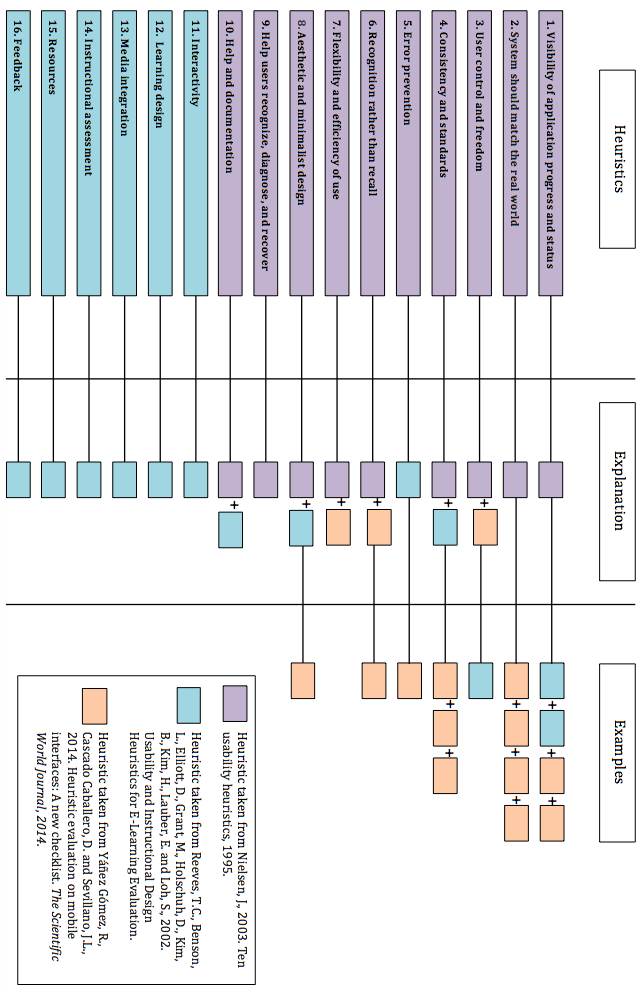
\includegraphics[width=1 \textwidth]{heu1}
\caption{Visual presentation on how the guideline has been constructed from \cite{nielsen199510}, \cite{reeves2002usability}, and \cite{yanez2014heuristic}}
\end{figure}

\subsection{Heuristic Evaluation of P1}

\textbf{Methodology}

In order to evaluate the P1 based on the heuristic guidelines, we invited seven experts to evaluate the P1. However, the evaluation did not based on the experts' ability but they were asked to role-play as a learner. 

In chapter 3, we gathered qualitative and quantitative data from real learners and created a model called persona. We also presented its contribution to successfully developing the P1. In this chapter, the same persona was also used as a user model for the role-play. In order to persuade the experts to get into the character, we rewrote the persona profile into storytelling.

\begin{figure}[!hbt]
\centering
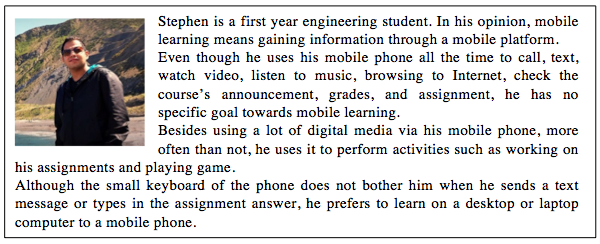
\includegraphics[width=1 \textwidth]{heu2}
\caption{The storytelling of the persona adopted from the primary persona presented in chapter 3}
\end{figure}

\cite{cooper2007face} claimed that understanding the three important keys: persona, goal, and scenario contributed to developing a good design. It was crucial to specify a learning goal, so that the experts could understand the purpose of learning and perform the role-played efficiently. 

Even though, the persona expressed that he did not have a specific goal towards m-learning, we formed a learning goal based on the findings in chapter 5 that the learners were motivated and had knowledge and skills to used the m-learning application. The learning goal explained what the persona wanted to feel, do, and achieve while he was using the application. The goal were: 
\begin{itemize}
\item Engage with the learning process, be entertained while learning, and be encouraged to learn. 
\item Use all the provided media, performed all the given learning activities, and learn all the provided learning content. 
\item Remember some of the learning content, and gain a better understanding towards the learning topic. 
\end{itemize} 

Besides the persona and the learning goals, we also specify a scenario for the experts. The scenario explained how the persona would use the m-learning application to achieve the learning goals. 

\cite{cooper2007face} explained that there were three types of scenario. The first scenario that should be formed at the beginning of the tool development was the context scenario. It explained in high level on how the tool was used in persona's daily activities. The key-path scenario was more descriptive on user-interaction. Therefore, it could be formed after a developer had primary defined the tool's function, and framework. The scenario explained on how the persona used the tool to achieve the learning goal. In particular, it described the how the persona interact with the tool's interface. The coming last scenario was the validation scenario. It was developed based on ``what if ...'' question used to test the design solution. 

The main purpose of the heuristic evaluation was to evaluate the interface design of P1, therefore we formed a key path scenario. In addition, we add some context into the scenario to make the story flow nicely and encourage the experts to perform the activities that we wanted to evaluate. The scenario were: 

\begin{enumerate}
\item While waiting for the next class to start, Stephen opens a new learning application that he downloaded last night. This is the first time he uses the application.
\item He skims through the types of available media and activities, and listens to the voice recording available from in the first screen of the application.
\item Then he watches the introduction video provided in the application. 
\item He starts to learn by reading the learning content in order and listens to all the available voice recordings at the first screen of each learning section. However, in the midst of this activity his class starts, so he quits from the application. 
\item After his class has finished, he re-opens the application and starts to learn the rest of the learning content. However, during this process, he has a question, so he contacts his supervisor. After he received a reply, he still wants to get extra information from the Internet.
\item Upon finishing learning all the content, he starts to play the provided game. In the middle of playing the game, Stephen wants to check his answer so he exits from the game to check the learning content. 
\item After he played the game a couple of times, he feels confident that he can recognize and understand the content. Therefore, he goes to the assignment screen, types in some short answers and submits the assignment to his supervisor. 
\end{enumerate} 

The experts, then were asked to perform the evaluation based on our heuristics guidelines. 

\textbf{Findings} - the following list is summary of the heuristic evaluation based on the heuristic guideline: 

\begin{enumerate}

\item Visibility of application progress and status - the application received a mixture of positive and negative comments for this guideline. 
For example, an expert who was satisfied with the visibility of the learning progress claimed that
\begin{addmargin}[1.5em]{1.5em}
\textit{``It's good at visual feedback and I could check my progress easily''}\end{addmargin} 

The other expert who was partially satisfied with the visibility commented that 
\begin{addmargin}[1.5em]{1.5em}
\textit{``It is partially there - I can see it during audio being played. However I find it difficult to see where I am up to within sections.''}\end{addmargin} 

On the other hand, there was an expert who thought the application failed to provide sufficient visibility commented that
\begin{addmargin}[1.5em]{1.5em}
\textit{``Progress through lessons was not clear. I was not sure where I was in the lesson or content.''}\end{addmargin} 

All things considered, there is still room for improvement to increase the visibility of application progress. The following list contains suggestions from the experts' on various approaches to enhance the application visibility: 
\begin{itemize}
\item Providing a consistent left hand menu that hierarchically display all learning pages and other activities pages, and use Breadcrumbs navigation (i.e., navigation scheme that reveals the learners' location where they are in the application). 
\item Consider adding audio to inform the status. For example, using audio to inform learners when whether they gain a point or lost a chance during the game
\item Providing an overview of all content to the learners while they are learning. 
\end{itemize}

\item System should match the real world- many of the comments proved that the application accomplished this guideline. The experts noted that there was consistent use of home, backward, and forward icons. They satisfied with how the learning content were divided in to sections and proper titled. In addition, they found that most words and phrases matched real world convention and easy to read. 

\item User control and freedom - the experts found major defects within the chat function. They reported that they were unable to leave the chat function and return to the home screen, and instead they had to reset the application and restart the testing process. Additionally, they provided many suggestions to improve the chat functionality: 

\begin{itemize} 
\item Give users the freedom to configure the chat app, such as adjust text size, ability to configure whether to hit enter key to send message (instead on click on ``send'' button)
\item Make entering the name compulsory so the name will display correctly in the app
\item Provide timestamps to inform the learners when the messages have been sent and received
\item Provide notifications and alerts about who has joined the chat
\item Using colour and layout to distinguish between learners and instructor 
\item Relocate the box to type in text and to send it to the chat room at bottom of the screen
\item Provide controllable keyboard (i.e., open and hide) 
\item Provide scrolling capabilities for learners so they can see the whole chat 
\end{itemize}

The experts also noted that we provided ``forward'' and ``backward'' button so that the learners could navigate themselves through the application. However, many of them encountered problems and provided some suggestions. For example, experts stated 
\begin{addmargin}[1.5em]{1.5em}
\textit{``I can easily use back arrows and home buttons and menus etc. to navigate around the application and go back and skip ahead, although the hierarchy and placement of menu needs to be more uniformed''}\end{addmargin}
\begin{addmargin}[1.5em]{1.5em}
\textit{``User control is good, I understand how I should work with it. Just a minor suggestion is all pages look similar to each other and this was a little confusing.''}\end{addmargin} 

Besides, we also received many suggestions on how the icon should be rearranged so that the learners could go through the learning lesson smoothly. For example, an expert suggested removing all unrelated icons from the chat page. Another expert suggest using text plus icon (we only provided icon in the application) to navigate the learners to ensure the accuracy. 

It has been shown that the experts acknowledged user control options we provided throughout the application. However, the current interface design (of the icons, titles, colours, and buttons) and defective performance (of the chat function) affected the experts' satisfaction and should be improved. 

\item Consistency and standard - we also received many comments against guideline. The following list contains the interface design issues we received from the experts: 
\begin{itemize}
\item The location of the "back" and "forward" buttons were not consistent 
\item The icons shown in the main menu and the other navigation screens were not consistent (i.e. missing the icons) 
\item The ``back'' button meant to navigate the learners to the previous page, but it brought them to another navigation page and caused confusion 
\item The background of many screens were distracting, including the cartoon character used in the application where should be dimmer or fade out and the text area with the lesson text should be wider
\item Text should be justified either left, right, or center consistently 
\item Every part of the learning content should be presented in the same template 
\item Many learning screen did not have title
\end{itemize}

Based on the comments and suggestions we received, the application failed to provide consistency or adhere to the design standard

\item Error prevention - when designing the application, we did not provide any error prevention mechanism. Hence, the experts were unable to comment on this guideline. 

\item Recognition rather than recall - majority of the experts were satisfied with the application design under this guideline. They did not need to remember any information from screen to screen. However, an expert pointed out that the application did not provide title for one of the learning section and this might require the learners to remember what they were learning. 

Another expert suggested including question in the e-mail for the assignment for learners, so that they did not need to remember the question or go back and forth between two screens when they are typing in the answer.

\item Flexibility and efficiency of use - the experts were considered as experienced users (They role-played the persona who had experienced using a mobile phone to performed many learning related activities). They found the application accommodated them well. Only one expert encountered with troubles learning on the application. S/he commented that 
\begin{addmargin}[1.5em]{1.5em}
\textit{``I think the design is good but it includes so many similar pages, which made me a little confusing. So I have to lead back to home to figure out the rest.''}\end{addmargin}

Regarding to the customization, we did not provide this option; therefore the experts were unable to provide any comment on it. 

\item Aesthetic and minimalist design - there were varied comments regarding to this guideline. An expert stated that s/he was satisfied with the application design and did not provide any further suggestions. However, other experts provided some further visual design suggestions. For example, an expert commented that the background of the text should be theme controlled throughout the application. 

Another expert who was partly satisfied with the application design comment that  
\begin{addmargin}[1.5em]{1.5em}
\textit{``I like the front page and the attractive first page - I think the app can be a bit bigger in terms of area of text displayed, and background image more faded to make text a bit more prominent. Icons and buttons are sufficient as needed so those are `succinct' enough.''}\end{addmargin}

and s/he further suggested that the combination of text and icon were more meaningful compared to only an icon. 

\item Help users recognize, diagnose, and recover from errors - unfortunately, many experts did not encounter any errors while they were using the application; therefore they were unable to comment on this guideline. They stated that
\begin{addmargin}[1.5em]{1.5em}
\textit{``I did not have problem with this section. It was fine.''}\end{addmargin}
\begin{addmargin}[1.5em]{1.5em}
\textit{``I encountered no error''}\end{addmargin} 

\item Help and documentation - we did not provide any help and support document. Nevertheless, most of the experts could learn on the application without any further help. For example, an expert claimed that  
\begin{addmargin}[1.5em]{1.5em}
\textit{``It had enough help and explanations to figure out what should be done next.''}\end{addmargin}

Even though, the expert found that the application was easy to use. Based on the guideline, the application should nevertheless provide some help for the learners. 

\item Interactivity - many experts satisfied with the interactivities provided in the application. For example they stated that 
\begin{addmargin}[1.5em]{1.5em}
\textit{``So interactive, I like playing with it'',}\end{addmargin}
\begin{addmargin}[1.5em]{1.5em}
\textit{``The combination of media and content felt good''}\end{addmargin}
\begin{addmargin}[1.5em]{1.5em}
\textit{``Audio, video and games content are available.''}\end{addmargin}

Besides the positive responses, we also receive some suggestions that could improve the interactivity of the application. For example, an expert who suggested improving the pop-up design interface stated that 
\begin{addmargin}[1.5em]{1.5em}
\textit{``Clicking on the text should also bring up the pop up as well as the explanation masks.''}\end{addmargin}

Based on the responses, the interactivity we provided in the application was appealing. However, its interface design could potentially be improved. 

\item Learning design - this guideline purposely guided the design of the application and was useful for the developers; therefore the experts who took the user role could not provide much qualitative comment on this guideline. The experts' comments were pretty broad: 
\begin{addmargin}[1.5em]{1.5em}
\textit{``Not sure about it since I don't know learning principles. But I could learn the stuff you provided in your application''}\end{addmargin}
\begin{addmargin}[1.5em]{1.5em}
\textit{``There are multimedia functions available to keep students interested.''}\end{addmargin} 

\item Media integration - many of the comments on the media integration were positive. For example, the experts claimed that
\begin{addmargin}[1.5em]{1.5em}
\textit{``Had media integrations''},\end{addmargin} 
\begin{addmargin}[1.5em]{1.5em}
\textit{``Media was instructional and useful''}\end{addmargin} 
\begin{addmargin}[1.5em]{1.5em}
\textit{``Agree that media are integrated correctly where needed.''}\end{addmargin} 

However, they found the technical problem with the audio media we provided. Many of the experts commented that 
\begin{addmargin}[1.5em]{1.5em}
\textit{``... any audio being played will continue to be played after the page has been exited''}\end{addmargin} 
\begin{addmargin}[1.5em]{1.5em}
\textit{``There is also no intuitive way of stopping the media afterwards''},\end{addmargin}
\begin{addmargin}[1.5em]{1.5em}
\textit{``Voice introduction is good, however if I press back \& go to other course and play a voice, it won't stop playing the first voice'.''}\end{addmargin}

We provided many media in the application (i.e., recorded voice, text, video). These media are deemed to be acceptable by the experts. However, the technical problem needed to be fixed. 

Even though the media variety seemed to impress many experts, an expert who found improper used media commented that 
\begin{addmargin}[1.5em]{1.5em}
\textit{``The media integration can be `placed' better within the application. (We have trouble understanding the relationship between the audio and the actual learning content – how they are different or overlap)''}\end{addmargin}

and further suggested repositioning some of the media in the application. 

\item Instructional assessment - unfortunately, we did not receive much qualitative comment on this guideline even though we provided a quiz game that aligned with the guideline (i.e., analysis type of question and asked the learners to express their opinion). 

\item Resources - the experts did not find any external link; therefor they were unable to comment on this guideline. 

\item Feedback - the experts found that the application provided feedback to the learners. 
For example, an expert stated that
\begin{addmargin}[1.5em]{1.5em}
\textit{``Successful in providing feedback since it let the users to contact the supervisor.''}\end{addmargin}

However, many of them commented that the feedback was not enough and suggested giving more feedback through audio media and using e-mail as communication medium. The responses were: 
\begin{addmargin}[1.5em]{1.5em}
\textit{``Very little feedback in the question and answer game some audio feedback would be nice.''}\end{addmargin}
\begin{addmargin}[1.5em]{1.5em}
\textit{``I noted that games gave out scoring, Chat function is also available to chat with peers and instructor. I don't see ability to email instruction directly though?''}\end{addmargin}
\end{enumerate}

The heuristic evaluation provided more insight feedback as the expert could raise some comments and suggests. In general, the responses from the heuristic evaluation were similar to the qualitative results we transcribed from the video (See chapter 4). The same technical problems occurred during the previous evaluation also found in the heuristic evaluation (e.g., could not exit out of chat function, and recorded voice did not automatically stop when the learners moved to the other screens). The experts expressed that they are satisfied with the media provided in the application. On the other hand, we received the most comments and suggestions on the interface design of the application. 

Notably, some heuristic evaluation guidelines were similar to what Transactional Distance Theory (TDT) had guide the design. For example, the theory suggested providing interactive media to attract learners to the learning content and this seemed to satisfy the experts. They claimed the media were useful and noted that many media were provided in the application. As evident from the responses received, the similar guidelines (e.g., system should match the real world, interactivity, and media integration) received satisfactory responses from the experts. 

On the other hand, the experts heavily criticised the consistency and standards of the design. They pointed out many interface design issues, and suggested how to improve the interface design of the application. This might be due in part to the intense focus on developing the application and its functionalities needed to achieve the TDT guidelines, and as a result neglected essential interface design principles. Beyond the theoretically based guideline, the heuristic guideline could assist in this gap. At a later stage of this research, we will present a new set of design guidelines, which will combine the two guidelines and eliminate any duplication.

Certainly, the application still needs some major re-design in areas such as information architecture and user interface. The application will be redesigned based on a new set of design guidelines, thus providing improvements aesthetically and structurally.

Notably, there were a few heuristic evaluation guidelines that the experts could not comment (i.e., learning design) on as they exist mainly to inform the development process. There were also many heuristic evaluation guidelines that the experts did not provide enough qualitative evaluation (e.g., instructional assessment and indicating error). Therefore, we (as a role of developer) will also evaluate the application using the same heuristic evaluation guideline to ensure the completeness of the evaluation and enhance the next application design. 

























